\documentclass[10pt]{article}
\usepackage[letterpaper, b3paper, landscape, margin=0.1in]{geometry}
\usepackage[utf8]{inputenc}		% LaTeX, comprend les accents !
\usepackage[T1]{fontenc}
\usepackage{natbib}	
%\usepackage[square,sort&compress,sectionbib]{natbib}		% Doit être chargé avant babel      
\usepackage[frenchb,english]{babel}
\usepackage{lmodern}
\usepackage{amsmath,amssymb, amsthm}
\usepackage[capposition=top]{floatrow}
\usepackage{verbatim}
\usepackage{float}
\usepackage{placeins}
\usepackage{flafter}
\usepackage{longtable}
\usepackage{import}
\usepackage{pdflscape}
\usepackage{rotating}
\usepackage{hhline}
\usepackage{multirow}
\usepackage{booktabs}
\usepackage[pdftex,pdfborder={0 0 0},colorlinks=true,linkcolor=blue,urlcolor=blue,citecolor=blue,bookmarksopen=true]{hyperref}
\usepackage{eurosym}
%\usepackage{breakcites}
\usepackage[autostyle]{csquotes}
%\usepackage{datetime}
\usepackage{natbib}
\usepackage{setspace}
\usepackage{lscape}
\usepackage[usenames]{color}
\usepackage{indentfirst}
\usepackage{url}
\usepackage{enumitem}
\usepackage{multirow}
\usepackage{subcaption}
\usepackage[justification=centering]{caption}
\bibliographystyle{agsm}
\usepackage{supertabular} 
\usepackage{array}

\usepackage{longtable}
\usepackage{longtable} % for 'longtable' environment
\usepackage{pdflscape} % for 'landscape' environment
\newcommand{\isEmbedded}{true}
\graphicspath{{Figures/}}


\begin{document}
	
	\selectlanguage{frenchb}





\begin{landscape}
	\begin{longtable}{ | p{0.5cm} |*{15}{c|} }

  % footer material
%taux de retention &  taux de retention si chgmt grade &  max taux de transition vers autre corps &             %autre corps ac. max taux de transition
& \textbf{(1)} & \textbf{(2)} & \textbf{(3)} & \textbf{(4)} & \textbf{(5)} & \textbf{(6)} & \textbf{(7)} & \textbf{(8)} & \textbf{(9)} & \textbf{(10)} \\
0   &                      Agents technique territoriaux &         336163 &          20.5\% &                  20.5\% &                17.0\% &                    17.0\% &              98.0\% &                             84.7\% &                                     1.2\% &                    Agents de maitrise territoriaux \\
1   &                                    Aides soignants &         178694 &          10.9\% &                  31.4\% &                 9.3\% &                    26.4\% &              98.9\% &                             81.7\% &                                     0.6\% &        Infirmiers en soins generaux et specialises \\
2   &               Adjoints administratifs territoriaux &         146233 &           8.9\% &                  40.3\% &                 7.5\% &                    33.9\% &              97.9\% &                             81.7\% &                                     1.4\% &                            Redacteurs territoriaux \\
3   &        Infirmiers en soins generaux et specialises &         105737 &           6.4\% &                  46.7\% &                 7.0\% &                    40.9\% &              98.7\% &                              nan\% &                                     0.4\% &                                         Infirmiers \\
4   &                                         Infirmiers &          77216 &           4.7\% &                  51.4\% &                 6.1\% &                    47.0\% &              98.4\% &                             64.3\% &                                     0.8\% &        Infirmiers en soins generaux et specialises \\
5   &         Agents des services hospitaliers qualifies &          60046 &           3.7\% &                  55.1\% &                 2.8\% &                    49.8\% &              96.1\% &                              nan\% &                                     2.9\% &                                    Aides soignants \\
6   &                            Redacteurs territoriaux &          38296 &           2.3\% &                  57.4\% &                 2.8\% &                    52.6\% &              97.5\% &                             78.1\% &                                     2.1\% &                              Attaches territoriaux \\
7   &                    Agents de maitrise territoriaux &          36755 &           2.2\% &                  59.7\% &                 2.4\% &                    57.7\% &              97.9\% &                             72.9\% &                                     1.8\% &                           Techniciens territoriaux \\
8   &               Adjoints administratifs hospitaliers &          34874 &           2.1\% &                  61.8\% &                 1.8\% &                    59.5\% &              98.9\% &                             78.2\% &                                     0.3\% &                               Secretaires medicaux \\
9   &                               Adjoints d animation &          31414 &           1.9\% &                  63.7\% &                 1.4\% &                    64.2\% &              97.0\% &                             63.2\% &                                     1.0\% &               Adjoints administratifs territoriaux \\
10  &                              Attaches territoriaux &          28216 &           1.7\% &                  65.4\% &                 2.7\% &                    55.3\% &              98.8\% &                             84.5\% &                                     0.8\% &                               Emplois fonctionnels \\
11  &  Agents territoriaux specialises des ecoles mat... &          26325 &           1.6\% &                  67.0\% &                 1.4\% &                    65.6\% &              98.5\% &                             92.2\% &                                     0.5\% &               Adjoints administratifs territoriaux \\
12  &                           Techniciens territoriaux &          23187 &           1.4\% &                  68.4\% &                 1.7\% &                    61.2\% &              97.9\% &                             75.9\% &                                     1.6\% &                                         Ingenieurs \\
13  &                            Ouvriers professionnels &          21194 &           1.3\% &                  69.7\% &                 1.1\% &                    70.4\% &              94.2\% &                              0.8\% &                                     4.5\% &                                   Maitres Ouvriers \\
14  &          Assistants territoriaux sociaux educatifs &          20310 &           1.2\% &                  71.0\% &                 1.5\% &                    62.8\% &              99.0\% &                             89.2\% &                                     0.3\% &         Conseillers territoriaux sociaux educatifs \\
15  &      Sapeurs pompiers professionnels non officiers &          17709 &           1.1\% &                  72.1\% &                 1.3\% &                    68.1\% &              99.5\% &                             93.0\% &                                     0.3\% &     Lieutenants de sapeurs pompiers professionnels \\
16  &           Auxiliaires de puericulture territoriaux &          17113 &           1.0\% &                  73.1\% &                 0.9\% &                    72.2\% &              98.5\% &                             92.7\% &                                     0.6\% &               Adjoints administratifs territoriaux \\
17  &                        Agents de police municipale &          14914 &           0.9\% &                  74.0\% &                 0.8\% &                    73.0\% &              98.9\% &                             90.7\% &                                     0.3\% &              Chefs de service de police municipale \\
18  &                        Agents sociaux territoriaux &          13513 &           0.8\% &                  74.8\% &                 0.6\% &                    74.9\% &              96.7\% &                             63.3\% &                                     0.7\% &                  Auxiliaires de soins territoriaux \\
19  &                                         Ingenieurs &          13366 &           0.8\% &                  75.6\% &                 1.3\% &                    66.9\% &              97.9\% &                             80.1\% &                                     1.6\% &                            Ingenieurs territoriaux \\
20  &                  Agents territoriaux du patrimoine &          12210 &           0.7\% &                  76.4\% &                 0.6\% &                    74.3\% &              98.0\% &                             81.4\% &                                     0.6\% &  Assistants de conservation du patrimoine et bi... \\
21  &                                 Agents d entretien &          11989 &           0.7\% &                  77.1\% &                 0.6\% &                    75.5\% &              91.9\% &                              nan\% &                                     6.1\% &                            Ouvriers professionnels \\
22  &                      Infirmiers surveillants chefs &          11893 &           0.7\% &                  77.8\% &                 1.2\% &                    69.3\% &              32.6\% &                              0.5\% &                                    66.9\% &                                     Cadre de sante \\
23  &                                   Maitres Ouvriers &          11780 &           0.7\% &                  78.6\% &                 0.7\% &                    73.7\% &              98.6\% &                             71.9\% &                                     0.9\% &                                      Contremaitres \\
24  &                                       Sages femmes &           9397 &           0.6\% &                  79.1\% &                 0.9\% &                    71.3\% &              99.7\% &                             93.6\% &                                     0.1\% &                         Sages femmes territoriales \\
25  &                  Auxiliaires de soins territoriaux &           7434 &           0.5\% &                  79.6\% &                 0.4\% &                    77.7\% &              98.4\% &                             88.6\% &                                     0.4\% &               Adjoints administratifs territoriaux \\
26  &  Educateur territoriaux des activites physiques... &           7343 &           0.4\% &                  80.0\% &                 0.5\% &                    76.0\% &              98.6\% &                             89.5\% &                                     0.4\% &                            Redacteurs territoriaux \\
27  &          Educateurs territoriaux de jeunes enfants &           6781 &           0.4\% &                  80.5\% &                 0.4\% &                    76.5\% &              98.3\% &                             94.2\% &                                     0.4\% &          Assistants territoriaux sociaux educatifs \\
28  &                            Animateurs territoriaux &           6390 &           0.4\% &                  80.8\% &                 0.4\% &                    76.9\% &              96.6\% &                             75.4\% &                                     1.6\% &                            Redacteurs territoriaux \\
29  &                         Assistants socio educatifs &           5753 &           0.4\% &                  81.2\% &                 0.4\% &                    77.3\% &              98.0\% &                              nan\% &                                     0.8\% &                                     Cadre de sante \\
30  &                       Puericultrices territoriales &           4223 &           0.3\% &                  81.4\% &                 0.4\% &                    78.0\% &              98.9\% &                             85.3\% &                                     0.4\% &                              Attaches territoriaux \\
31  &                                       Psychologues &           3680 &           0.2\% &                  81.7\% &                 0.3\% &                    78.7\% &              99.7\% &                             92.7\% &                                     0.1\% &                                    Aides soignants \\
32  &  Assistants de conservation du patrimoine et bi... &           3605 &           0.2\% &                  81.9\% &                 0.3\% &                    80.3\% &              98.7\% &                             89.6\% &                                     0.4\% &                       Bibliothecaires territoriaux \\
33  &                                      Contremaitres &           3508 &           0.2\% &                  82.1\% &                 0.2\% &                    80.6\% &              98.0\% &                             66.7\% &                                     1.2\% &                                   Maitres Ouvriers \\
34  &                            Infirmiers territoriaux &           3449 &           0.2\% &                  82.3\% &                 0.3\% &                    80.1\% &              32.7\% &                              7.6\% &                                    64.3\% &                        Infirmier en soins generaux \\
35  &   Infirmiers specialises en anesthesie reanimation &           3218 &           0.2\% &                  82.5\% &                 0.3\% &                    78.4\% &              99.3\% &                             83.3\% &                                     0.2\% &                                     Cadre de sante \\
36  &                                     Puericultrices &           3060 &           0.2\% &                  82.7\% &                 0.3\% &                    79.8\% &              97.6\% &                             53.2\% &                                     1.4\% &                       Puericultrices territoriales \\
37  &  Professeurs territoriaux d enseignement artist... &           2777 &           0.2\% &                  82.9\% &                 0.3\% &                    79.3\% &              99.5\% &                             91.5\% &                                     0.3\% &  Directeurs d etablissements d enseignement art... \\
38  &                           Conducteurs ambulanciers &           2774 &           0.2\% &                  83.0\% &                 0.2\% &                    81.8\% &              98.7\% &                             78.1\% &                                     0.5\% &                                    Aides soignants \\
39  &                               Secretaires medicaux &           2570 &           0.2\% &                  83.2\% &                 0.2\% &                    81.3\% &              97.9\% &                             70.0\% &                                     1.0\% &                                    Aides soignants \\
40  &          Sapeurs pompiers professionnels officiers &           2521 &           0.2\% &                  83.3\% &                 0.3\% &                    79.0\% &              99.7\% &                             95.6\% &                                     0.2\% &                        Infirmier en soins generaux \\
41  &                               Moniteurs educateurs &           2426 &           0.1\% &                  83.5\% &                 0.1\% &                    82.3\% &              96.9\% &                              nan\% &                                     2.3\% &                         Assistants socio educatifs \\
42  &                               Emplois fonctionnels &           2282 &           0.1\% &                  83.6\% &                 0.3\% &                    79.6\% &              92.8\% &                             22.5\% &                                     4.8\% &                              Attaches territoriaux \\
43  &     Lieutenants de sapeurs pompiers professionnels &           2187 &           0.1\% &                  83.8\% &                 0.2\% &                    80.8\% &              95.0\% &                             78.4\% &                                     4.9\% &          Sapeurs pompiers professionnels officiers \\
44  &                    Infirmiers de salle d operation &           2075 &           0.1\% &                  83.9\% &                 0.2\% &                    81.0\% &              99.0\% &                             80.8\% &                                     0.3\% &                                     Cadre de sante \\
45  &           Manipulateurs electroradiologie medicale &           2073 &           0.1\% &                  84.0\% &                 0.2\% &                    81.5\% &              99.4\% &                             88.7\% &                                     0.3\% &  Manipulateurs electroradiologie surveillants c... \\
46  &                         Techniciens de laboratoire &           1807 &           0.1\% &                  84.1\% &                 0.2\% &                    82.0\% &              99.5\% &                             93.4\% &                                     0.2\% &      Techniciens de laboratoire surveillants chefs \\
47  &         Conseillers territoriaux sociaux educatifs &           1797 &           0.1\% &                  84.2\% &                 0.1\% &                    82.4\% &              90.6\% &                              nan\% &                                     4.2\% &                              Attaches territoriaux \\
48  &                            Ingenieurs hospitaliers &           1697 &           0.1\% &                  84.3\% &                 0.2\% &                    81.1\% &              99.2\% &                             91.7\% &                                     0.2\% &                                         Ingenieurs \\
49  &  Assistants territoriaux d enseignement artistique &           1380 &           0.1\% &                  84.4\% &                 0.1\% &                    82.8\% &              98.5\% &                              nan\% &                                     0.7\% &  Professeurs territoriaux d enseignement artist... \\
50  &                              Medecins territoriaux &           1273 &           0.1\% &                  84.5\% &                 0.2\% &                    81.7\% &              93.5\% &                             63.4\% &                                     6.2\% &  Agents territoriaux specialises des ecoles mat... \\
51  &                       Bibliothecaires territoriaux &           1204 &           0.1\% &                  84.6\% &                 0.1\% &                    82.7\% &              98.9\% &                              nan\% &                                     0.6\% &                              Attaches territoriaux \\
52  &                                    Chefs de bureau &           1135 &           0.1\% &                  84.6\% &                 0.1\% &                    82.6\% &              98.7\% &                             72.0\% &                                     0.5\% &                              Attaches territoriaux \\
53  &                            Animateurs hospitaliers &           1128 &           0.1\% &                  84.7\% &                 0.1\% &                    83.5\% &              99.0\% &                              nan\% &                                     0.4\% &                            Animateurs territoriaux \\
54  &                       Educateurs de jeunes enfants &           1112 &           0.1\% &                  84.8\% &                 0.1\% &                    83.3\% &              98.5\% &                             85.2\% &                                     0.6\% &          Educateurs territoriaux de jeunes enfants \\
55  &   Assistants territoriaux qualifies de laboratoire &           1084 &           0.1\% &                  84.9\% &                 0.1\% &                    83.1\% &               nan\% &                              nan\% &                                    91.6\% &                             Technicien paramedical \\
56  &                   Adjoints des cadres hospitaliers &           1057 &           0.1\% &                  84.9\% &                 0.1\% &                    83.2\% &              97.1\% &                              7.1\% &                                     2.2\% &                                    Chefs de bureau \\
57  &                            Ingenieurs territoriaux &           1010 &           0.1\% &                  85.0\% &                 0.1\% &                    82.1\% &              98.0\% &                             67.7\% &                                     1.4\% &                               Emplois fonctionnels \\
58  &   Attaches territoriaux de conservation patrimoine &           1002 &           0.1\% &                  85.0\% &                 0.1\% &                    82.9\% &              98.0\% &                              nan\% &                                     0.6\% &                              Attaches territoriaux \\
59  &                           Psychologue territoriaux &            968 &           0.1\% &                  85.1\% &                 0.1\% &                    83.0\% &              98.6\% &                             82.7\% &                                     0.4\% &                                       Psychologues \\
60  &              Chefs de service de police municipale &            962 &           0.1\% &                  85.2\% &                 0.1\% &                    83.4\% &              98.7\% &                             94.3\% &                                     0.6\% &                        Agents de police municipale \\
61  &                          Preparateurs en pharmacie &            878 &           0.1\% &                  85.2\% &                 0.1\% &                    83.6\% &              99.8\% &                             93.1\% &                                     0.1\% &                                         Infirmiers \\
62  &  Operateurs territoriaux des activites physique... &            848 &           0.1\% &                  85.3\% &                 0.0\% &                    84.2\% &              96.5\% &                             78.6\% &                                     2.6\% &  Educateur territoriaux des activites physiques... \\
63  &                         Masseurs kinesitherapeutes &            839 &           0.1\% &                  85.3\% &                 0.1\% &                    83.7\% &              99.2\% &                             76.0\% &                                     0.1\% &               Adjoints administratifs territoriaux \\
64  &                      Directeur general sur contrat &            825 &           0.1\% &                  85.4\% &                 0.1\% &                    82.5\% &              99.5\% &                              nan\% &                                     0.5\% &         Personnel direction etablissements sociaux \\
65  &                              Secretaires de mairie &            758 &           0.0\% &                  85.4\% &                 0.1\% &                    83.5\% &              89.4\% &                              nan\% &                                     4.8\% &                              Attaches territoriaux \\
66  &         Personnel direction etablissements sociaux &            752 &           0.0\% &                  85.5\% &                 0.1\% &                    83.2\% &              95.0\% &                             68.2\% &                                     2.3\% &                            Personnels de direction \\
67  &  Assistants territoriaux specialises d enseigne... &            688 &           0.0\% &                  85.5\% &                 0.1\% &                    83.9\% &               nan\% &                              nan\% &                                    85.9\% &  Assistants territoriaux d enseignement artistique \\
68  &                  Puericultrices surveillants chefs &            571 &           0.0\% &                  85.5\% &                 0.1\% &                    83.7\% &              20.0\% &                              0.9\% &                                    79.3\% &                                     Cadre de sante \\
69  &  Conseillers territoriaux des activites physiqu... &            548 &           0.0\% &                  85.6\% &                 0.1\% &                    84.1\% &              82.7\% &                              7.1\% &                                    12.9\% &                              Attaches territoriaux \\
70  &                         Sages femmes territoriales &            519 &           0.0\% &                  85.6\% &                 0.1\% &                    84.0\% &              99.6\% &                             96.2\% &                                     0.4\% &                                       Sages femmes \\
71  &  Manipulateurs electroradiologie surveillants c... &            515 &           0.0\% &                  85.6\% &                 0.1\% &                    84.0\% &              26.3\% &                              0.5\% &                                    73.3\% &                                     Cadre de sante \\
72  &                            Personnels de direction &            490 &           0.0\% &                  85.7\% &                 0.1\% &                    83.9\% &              83.2\% &                              2.5\% &                                    15.1\% &                      Directeur general sur contrat \\
73  &                        Administrateur territoriaux &            489 &           0.0\% &                  85.7\% &                 0.1\% &                    83.8\% &              93.0\% &                             40.4\% &                                     5.2\% &                               Emplois fonctionnels \\
74  &                                    Ergotherapeutes &            481 &           0.0\% &                  85.7\% &                 0.0\% &                    84.3\% &              98.1\% &                             42.9\% &                                     0.7\% &                             Technicien paramedical \\
75  &                                     Cadre de sante &            459 &           0.0\% &                  85.7\% &                 0.0\% &                    84.3\% &              98.6\% &                             53.8\% &                                     0.5\% &         Conseillers territoriaux sociaux educatifs \\
76  &  Infirmiers anesthesistes reanimation surveilla... &            458 &           0.0\% &                  85.8\% &                 0.1\% &                    84.1\% &              28.2\% &                              0.9\% &                                    70.9\% &                                     Cadre de sante \\
77  &  Infirmiers de salle d operation surveillants c... &            420 &           0.0\% &                  85.8\% &                 0.0\% &                    84.2\% &              29.5\% &                              0.4\% &                                    70.2\% &                                     Cadre de sante \\
78  &                                  Gardes champetres &            400 &           0.0\% &                  85.8\% &                 0.0\% &                    84.5\% &              97.4\% &                             85.5\% &                                     1.8\% &                        Agents de police municipale \\
79  &                  Educateurs techniques specialises &            394 &           0.0\% &                  85.8\% &                 0.0\% &                    84.4\% &              99.5\% &                             87.5\% &                                     0.3\% &                         Assistants socio educatifs \\
80  &      Techniciens de laboratoire surveillants chefs &            372 &           0.0\% &                  85.9\% &                 0.0\% &                    84.3\% &              20.8\% &                              nan\% &                                    78.7\% &                                     Cadre de sante \\
81  &                                       Dieteticiens &            369 &           0.0\% &                  85.9\% &                 0.0\% &                    84.4\% &              99.4\% &                             84.6\% &                                     0.3\% &                                     Cadre de sante \\
82  &                                   Psychomotriciens &            368 &           0.0\% &                  85.9\% &                 0.0\% &                    84.4\% &              99.4\% &                             83.3\% &                                     0.3\% &        Infirmiers en soins generaux et specialises \\
83  &                                Moniteurs d atelier &            336 &           0.0\% &                  85.9\% &                 0.0\% &                    84.6\% &              98.1\% &                              nan\% &                                     1.9\% &                  Educateurs techniques specialises \\
84  &   Permanenciers auxiliaires de regulation medicale &            313 &           0.0\% &                  86.0\% &                 0.0\% &                    84.6\% &              77.3\% &                             14.7\% &                                    16.0\% &                               Secretaires medicaux \\
85  &  Assistants territoriaux qualifies de conservation &            309 &           0.0\% &                  86.0\% &                 0.0\% &                    84.5\% &               nan\% &                              nan\% &                                    93.5\% &  Assistants de conservation du patrimoine et bi... \\
86  &       Conseillers en economie sociale et familiale &            307 &           0.0\% &                  86.0\% &                 0.0\% &                    84.5\% &              99.0\% &                             86.4\% &                                     0.3\% &                   Adjoints des cadres hospitaliers \\
87  &           Conservateurs territoriaux de patrimoine &            283 &           0.0\% &                  86.0\% &                 0.0\% &                    84.4\% &              94.4\% &                             37.5\% &                                     3.8\% &         Conservateurs territoriaux de bibliotheque \\
88  &                          Reeducateurs territoriaux &            278 &           0.0\% &                  86.0\% &                 0.0\% &                    84.6\% &               nan\% &                              nan\% &                                    92.3\% &                             Technicien paramedical \\
89  &         Conservateurs territoriaux de bibliotheque &            206 &           0.0\% &                  86.0\% &                 0.0\% &                    84.5\% &              94.2\% &                             47.6\% &                                     2.6\% &           Conservateurs territoriaux de patrimoine \\
90  &      Masseurs kinesitherapeutes surveillants chefs &            200 &           0.0\% &                  86.1\% &                 0.0\% &                    84.6\% &              32.6\% &                              nan\% &                                    66.8\% &                                     Cadre de sante \\
91  &            Preparateur en pharmacie cadre de sante &            175 &           0.0\% &                  86.1\% &                 0.0\% &                    84.6\% &              20.5\% &                              nan\% &                                    79.5\% &                                     Cadre de sante \\
92  &                                       Agents chefs &            175 &           0.0\% &                  86.1\% &                 0.0\% &                    84.7\% &              98.8\% &                             71.4\% &                                     0.6\% &                                Adjoints techniques \\
93  &                                     Orthophonistes &            172 &           0.0\% &                  86.1\% &                 0.0\% &                    84.7\% &             100.0\% &                            100.0\% &                                     nan\% &                                                NaN \\
94  &                                Adjoints techniques &            162 &           0.0\% &                  86.1\% &                 0.0\% &                    84.7\% &              99.3\% &                              nan\% &                                     0.7\% &                           Techniciens territoriaux \\
95  &                  Moniteurs-educateurs territoriaux &            130 &           0.0\% &                  86.1\% &                 0.0\% &                    84.7\% &              93.3\% &                              nan\% &                                     4.2\% &                            Redacteurs territoriaux \\
96  &                Directeurs des ecoles paramedicales &            117 &           0.0\% &                  86.1\% &                 0.0\% &                    84.6\% &              99.0\% &                             95.0\% &                                     1.0\% &                      Agents technique territoriaux \\
97  &                               Aides de laboratoire &            114 &           0.0\% &                  86.1\% &                 0.0\% &                    84.7\% &              95.5\% &                              nan\% &                                     2.7\% &                                   Maitres Ouvriers \\
98  &                              Agents d amphitheatre &            105 &           0.0\% &                  86.1\% &                 0.0\% &                    84.7\% &              96.0\% &                              nan\% &                                     1.0\% &               Adjoints administratifs hospitaliers \\
99  &                                 Aides de pharmacie &             83 &           0.0\% &                  86.1\% &                 0.0\% &                    84.7\% &              95.1\% &                             20.0\% &                                     2.4\% &                                    Aides soignants \\
100 &                                       Dessinateurs &             83 &           0.0\% &                  86.1\% &                 0.0\% &                    84.7\% &              98.7\% &                             80.0\% &                                     1.3\% &                            Personnels de direction \\
101 &                    Dieteticiens surveillants chefs &             78 &           0.0\% &                  86.1\% &                 0.0\% &                    84.7\% &              20.5\% &                              nan\% &                                    78.1\% &                                     Cadre de sante \\
102 &                 Ergotherapeutes surveillants chefs &             66 &           0.0\% &                  86.1\% &                 0.0\% &                    84.7\% &              12.9\% &                              nan\% &                                    85.5\% &                                     Cadre de sante \\
103 &  Directeurs d etablissements d enseignement art... &             54 &           0.0\% &                  86.1\% &                 0.0\% &                    84.7\% &              96.1\% &                             50.0\% &                                     2.0\% &                        Administrateur territoriaux \\
104 &                                       Orthoptistes &             50 &           0.0\% &                  86.1\% &                 0.0\% &                    84.7\% &              98.0\% &                             50.0\% &                                     2.0\% &                                     Orthophonistes \\
105 &                              Agents administratifs &             39 &           0.0\% &                  86.1\% &                 0.0\% &                    84.7\% &              85.7\% &                              nan\% &                                     5.7\% &               Adjoints administratifs hospitaliers \\
106 &                                  Emplois nationaux &             35 &           0.0\% &                  86.2\% &                 0.0\% &                    84.7\% &             100.0\% &                              nan\% &                                     nan\% &                                                NaN \\
107 &                Psychomotriciens surveillants chefs &             20 &           0.0\% &                  86.2\% &                 0.0\% &                    84.7\% &              22.2\% &                              nan\% &                                    72.2\% &                                     Cadre de sante \\
108 &                      Agents techniques d entretien &             18 &           0.0\% &                  86.2\% &                 0.0\% &                    84.7\% &              83.3\% &                              nan\% &                                    16.7\% &                                      Contremaitres \\
109 &                 Directeurs d ecole de sages femmes &             15 &           0.0\% &                  86.2\% &                 0.0\% &                    84.7\% &             100.0\% &                              nan\% &                                     nan\% &                                                NaN \\
110 &                  Orthophonistes surveillants chefs &              7 &           0.0\% &                  86.2\% &                 0.0\% &                    84.7\% &              42.9\% &                              nan\% &                                    57.1\% &                                     Cadre de sante \\
111 &                               Pedicures podologues &              4 &           0.0\% &                  86.2\% &                 0.0\% &                    84.7\% &             100.0\% &                              nan\% &                                     nan\% &                                                NaN \\
112 &                            Conducteurs automobiles &              3 &           0.0\% &                  86.2\% &                 0.0\% &                    84.7\% &              66.7\% &                              nan\% &                                    33.3\% &                                   Maitres Ouvriers \\
113 &                                      Standardistes &              3 &           0.0\% &                  86.2\% &                 0.0\% &                    84.7\% &              66.7\% &                              nan\% &                                    33.3\% &               Adjoints administratifs hospitaliers \\
114 &            Pedicures podologues surveillants chefs &              1 &           0.0\% &                  86.2\% &                 0.0\% &                    84.7\% &               nan\% &                              nan\% &                                   100.0\% &                                     Cadre de sante \\
115 &                             Technicien paramedical &              1 &           0.0\% &                  86.2\% &                 0.0\% &                    84.7\% &             100.0\% &                              nan\% &                                     nan\% &                                                NaN \\
	    &                              Total ou Moyenne				 &      1 413 672 & 86.2\% & 86.2\% & 84.7 \% & 84.7 \% & 88.1\% & 66.6\% & 14.9 \%
	\end{longtable}
\indent \textsc{Colonnes :}

\begin{itemize}
	\item \textbf{(1)} Label du corps d'appartenance en 2012
	\item \textbf{(2)} Effectifs par corps en 2012
	\item \textbf{(3)} Part du total des effectifs de 2012
	\item \textbf{(4)} Part cumulée du total des effectifs de 2012
	\item \textbf{(5)} Part de la somme des indices bruts de 2012
	\item \textbf{(6)} Part cumulée de la somme des indices bruts de 2012
	\item \textbf{(7)} Taux de rétention dans le corps entre 2012 et 2013
	\item \textbf{(8)} Taux de rétention entre 2012 et 2013 parmi les agents qui changent de grade entre 2012 et 2013 
	\item \textbf{(9)} Taux de transition maximum vers un autre corps en 2013
	\item \textbf{(10)} Corps 2013 différent du corps de 2012 vers lequel il y a le plus de transitions
\end{itemize}
\indent \indent \textsc{Population:} Individus qui ont leur code grade CIR renseigné pour les deux années 2012 et 2013 (1 640 850 identifiants contre 2 058 445 au total). 1 308 996 agents restent dans un même corps entre 2012 et 2013. 116 corps sont représentés. 14 \% des agents ne peuvent pas être rattachés à un corps car leur code cir n'est pas présent dans la table de correspondance que l'on a.\\
\indent \textsc{Lecture:} Il y a 3 36 163 Agents techniques territoriaux en 2012, ce qui représente 20.5 \% des effectifs de 2012 (restreints aux agents ayant leur code cir renseigné pour les deux années 2012 2013) et 20.5 \% des effectifs cumulés décroissants car c'est le corps où il y a le plus grand nombre d'agents. 98 \% des agents qui sont dans le corps des ATT en 2012 y sont également en 2013. 84.7 \% des agents qui sont dans le corps des ATT en 2012 et qui changent de grade entre 2012 et 2013 restent tout de même à l'intérieur du corps des ATT. Le corps qui en 2013 reçoit le plus d'agents venant du corps ATT est le corps des Agents de maîtrise territoriaux (1.2\% des agents qui sont en 2012 dans le corps ATT sont en 2013 dans le corps des Agents de maîtrise territoriaux).\\
\indent \textsc{Note 1:} Les NaN dans les colonnes taux de rétention, taux de rétention condit. à chgmt de grade et Max. des taux de transit. vers d'autres corps devraient être des 0.
\indent \textsc{Note 2:} La somme totale des indices bruts de 2012 est 597 770 300, avec une moyenne de 44 245 562 par corps environ. Le corps qui a la somme d'indices brutes la plus importante en 2012 est ATT avec 101 882 294, soit environ 17 pourcents du total.\\
\indent \textsc{Note 3:} Le tableau est trié par effectifs décroissants, ce qui explique que la colonne des ib cumulées ne soit pas exactement ordonnée.\\


\begin{figure}[H] 
	\caption{Relation entre taux de rétention de chaque corps entre 2012 et 2013 et effectifs dans le corps en 2012.}
	\label{transit1} 
	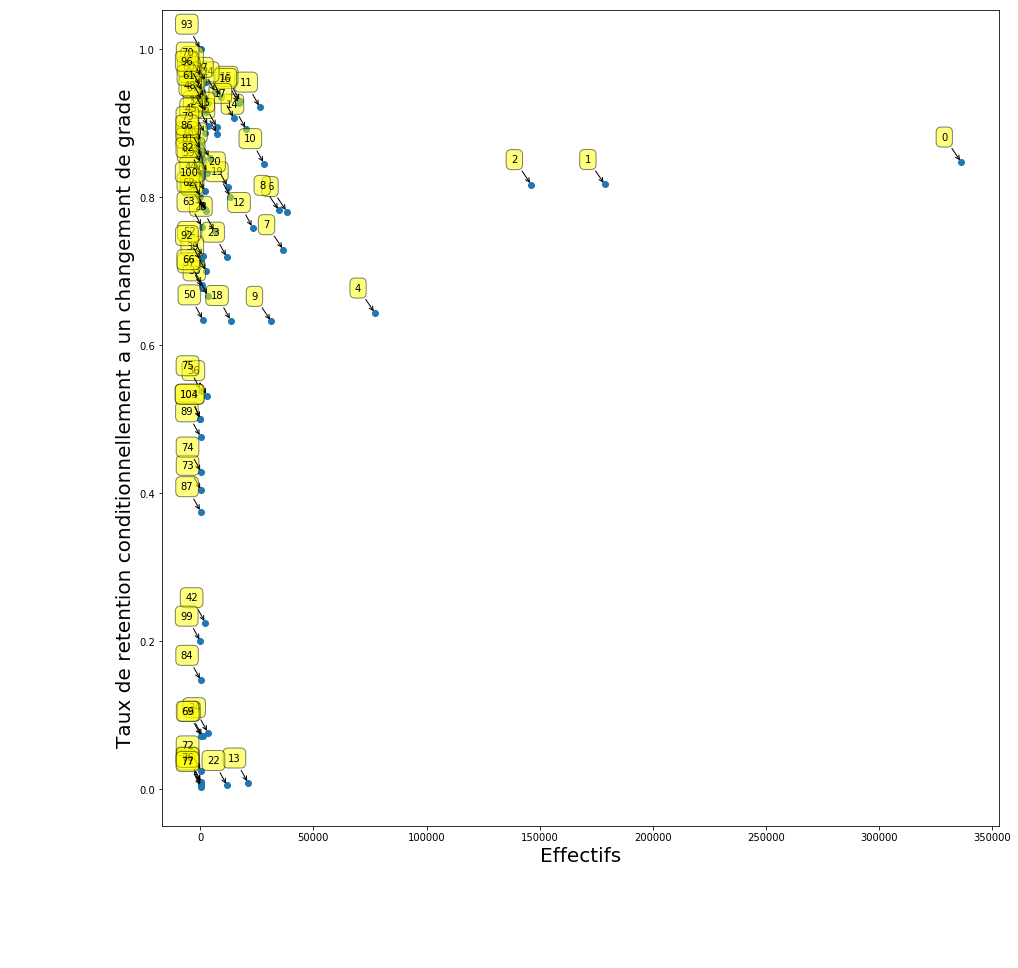
\includegraphics[scale = 0.7]{effectifs_tx_retentions_cdt_chgmt_grade.png} 
\end{figure}

	\textsc{Population:} Individus qui ont leur code grade CIR renseigné pour les deux années 2012 et 2013 (1 640 850 identifiants contre 2 058 445 au total) restreint aux agents qui changent de grade entre 2012 et 2013 (200 350).\\
	\indent \textsc{Lecture:} Le corps numéroté 0, i.e le corps des ATT, est très peuplé (environ 330 000 agents) en 2012 et a un très fort taux de rétention des agents qui changent de grades entre 2012 et 2013 (environ 90 \% des agents étant dans le corps des ATT en 2012 et changeant de grade entre 2012 et 2013 le font à l'intérieur du corps des ATT). \\
	\indent \textsc{Note:} Les numéros des points correspondent aux numéros de ligne dans le tableau ci-dessus, ce qui permet de retrouver le nom du corps.

 
\pagebreak


\begin{figure}[H] 
	\caption{Fréquences des differents taux de retention conditionnels à un changement de grade}
	\label{transit1} 
	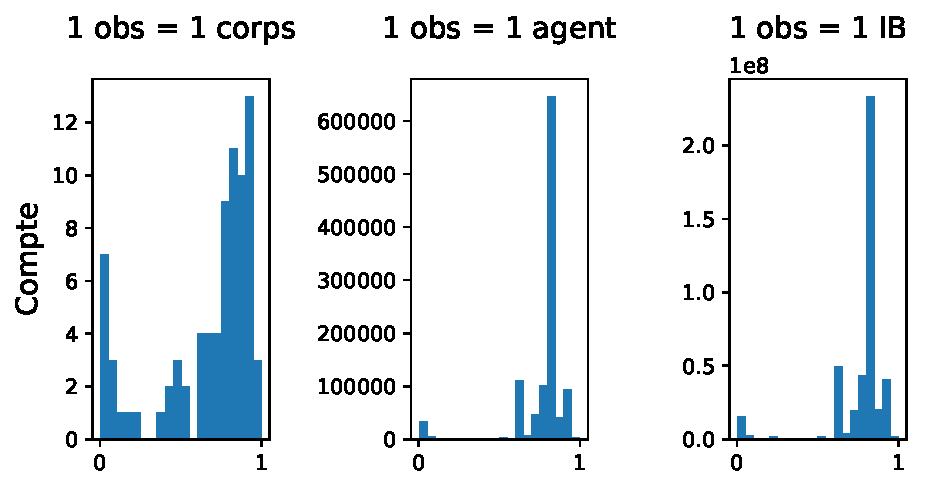
\includegraphics[scale = 1]{hist_tx_retention_conditionnels.pdf} 
\end{figure}
\center
\begin{minipage}{18cm}
\indent \textsc{Lecture :} 7 corps ont  un taux de rétention conditionnel à un changement de grade d'environ 0. Toutefois, 600 000 agents sont dans des corps ayant un taux de rétention parmi les agens qui changent de grade entre 2012 et 2013 d'environ 0.9. Environ 230 millions d'indices bruts de 2012 appartiennent à des corps ayant un taux de rétention conditionnellement à un changement de grade d'environ 0.9.
\end{minipage}

\end{landscape}




\end{document}